\documentclass[homework]{IEEEtran}
\IEEEoverridecommandlockouts
% The preceding line is only needed to identify funding in the first footnote. If that is unneeded, please comment it out.
\usepackage{cite}
\usepackage{CJKutf8}
\usepackage{indentfirst}
\usepackage{amsmath,amssymb,amsfonts}
\usepackage{algorithmic}
\usepackage{graphicx}
\usepackage{textcomp}
\usepackage{xcolor}
\usepackage{hyperref}
\usepackage[justification=centering]{caption}
\setlength{\parindent}{2em}
\def\BibTeX{{\rm B\kern-.05em{\sc i\kern-.025em b}\kern-.08em
    T\kern-.1667em\lower.7ex\hbox{E}\kern-.125emX}}
\begin{document}

\title{Homework of Pattern classification IV\\
{\footnotesize \textsuperscript{*}Name: Xue Yuan  | Student number: 202228015926034}
}

\author{}
\maketitle

\begin{abstract}
This document is about the first homework for Pattern classification by \LaTeX.
\end{abstract}

\section{Short Answers and Descriptions}
\begin{CJK}{UTF8}{gkai}
$\mathbf{Q1}$: 简述PCA的原理、学习模型和算法步骤。 \par
$\mathbf{A1}$: PCA原理:PCA全称为Principal Component Analysis,是一种无监督的学习方法,其主要目的是在对原样本降维后尽可能的保持其原有空间特性(差异性)。
它通过一个映射矩阵,将原有高维空间映射至一个较低维度的空间之中,并提取其特征,用新空间较低维度的特征来描述原样本的性质。 \par
$\mathbf{A2}$:PCA模型:我们用样本在m某维特征上的方差来定义特征的重要性,样本在这一特征上的差异越大,意味着该特征越能体现样本之间的差异,越有利于保留原始空间的差异性特征,也就越重要。
\begin{align*}
\mathbf{U} &= \left[ u_1,u_2, \dots,u_d \right]^T \in R^d \quad  \text{d维原始特征空间} \\
\mathbf{V} &= \left[ v_1,v_2, \dots,v_m \right]^T \in R^m \quad \text{m维新特征空间}
\end{align*} \par
设有转换矩阵W满足:
$$
v_i = \sum\limits_{j=1}^{d}w_{ij}\mu_{j}=W(:,i)^TU, i=1,2,\dots,m
$$\par
其中,$W(:,i)$代表矩阵W的第i列。有归一化条件:
$$
W(:,i)^TW(:,i)=1
$$
以样本对$v_1$的方差为例:
\begin{align*}
Var(v_1) &= E(v_{1}^{2}) - E(v_1)^2 \\
		  &=E\left(W(:,1)^TUU^TW(:,1)\right) \\
          &-E\left(W(:,1)^TU \right)E\left(W(:,1)U^T\right) \\
		  &= W(:,1)^T \left(E(UU^T)-E(U)E(U^T) \right)W(:,1)
\end{align*}\par
不妨令:
$$
W(:,1) = \alpha, \dot E(UU^T)-E(U)E(U^T) = \Sigma
$$\par
则原问题变换为求解下列最优化问题:
\begin{align*}
&\max_{\alpha} \alpha^T \Sigma \alpha \\
&s.t. \quad \alpha^T \alpha =1
\end{align*}\par
引入拉格朗日乘子构造拉格朗日函数有:
$$
L(\alpha) = \alpha^T \Sigma \alpha - \lambda(\alpha^T \alpha -1)
$$\par
分别求导可得:
\begin{align*}
\frac{\partial L}{\partial \alpha} &=\Sigma \alpha-\lambda \alpha=0 \\
\frac{\partial L}{\partial \lambda}&=\alpha^{T} \alpha-1=0
\end{align*}\par
则,$\lambda$和$\alpha$分别可以视为协方差矩阵$\Sigma$的特征值和相对应的特征向量。因此,原优化目标可以带换为:
$$
\max =  \alpha^T \Sigma \alpha =\alpha^T(\lambda \alpha) = \lambda
$$\par
即求协方差矩阵特征值的最大值,而$W(:,1)$为协方差矩阵所对应的特征向量,如下式:
$$
\Sigma W(:,1)=\lambda_1 W(:,1)
$$\par
同理,转换矩阵的第i列$W(:,i)$w就为数据协方差矩阵的第i大特征值所对应的特征向量。\par
由此,可以总结PCA算法的学习模型:对数据的协方差矩阵做特征值分解,将特征值按从大到小顺序排列,取前k个最大特征值对应的特征
向量作为特征向量的主成分,构造转换矩阵$W(:,i)$,再同通过$y_{i}=W^{T}\left(x_{i}-\mu\right)$对原样本进行降维,提取特征。\par
$\mathbf{Q3}$:PCA的算法步骤可以由下过程表示: \par
输入: 样本集合$X$,主成分个数$k$ \par
输出: 线性变换矩阵$W$,均值向量$\mu$,降维后样本集合$Y$ \par
\begin{enumerate}
\item 计算样本均值: $ \mu=\sum_{i=1}^{N} x_{i} $
\item 计算样本离散度矩阵:$S=\sum_{i=1}^{N}\left(x_{i}-\mu\right)\left(x_{i}-\mu\right)^{T}$ 
\item 对离散度矩阵$\mathrm{S}$进行特征值分解,取前$k$个最大的特征值对应的特征向量组成线性变换矩阵$W$,其中$W$的第$i$列对应第$i$个特征向量。
\item 对输入样本进行降维:$y_{i}=W^{T}\left(x_{i}-\mu\right) $
\end{enumerate}

$\mathbf{Q2}$:简述LDA的原理和学习模型,给出多类LDA的计算步骤。\par
$\mathbf{A1}$:与PCA类似,LDA的目的也是为了将原始的高维数据映射至一个低维的特征空间之中。不同之处则在于LDA是一种监督学习,学习的目的是
为了最大化数据的线性可分性,提高分类性能。\par
LDA通常采用Fisher判别准则,故又通常被称为FDA,其基本思路就是为了使变化后的特征类内散度尽量小,而类间散度尽量大。假设有$C$类样本,
第$i$类样本个数是$N_{i}$,$m_{i}$是第$i$类样本的均值,$x_{j}^{i}$表示第$i$类中第$j$个样本,$m$是所有样本的均值,定义:
\begin{align*}
\text{类内散度}  \quad S w &=\sum_{i=1}^{C} \sum_{j=1}^{N_{i}}\left(x_{j}^{i}-m_{i}\right)\left(x_{j}^{i}-m_{i}\right)^{T} \\
\text{类间散度}  \quad S b &=\sum_{i=1}^{C} N_{i}\left(m_{i}-m\right)\left(m_{i}-m\right)^{T} \\
\text{总体散度}  \quad S t &=\sum_{i=i}^{C} \sum_{j=1}^{N_{i}}\left(x_{j}^{i}-m\right)\left(x_{j}^{i}-m\right)^{T} 
\end{align*} \par
假设存在线性变换矩阵W,使$y=W^Tx$成立,则变换后的低维空间中,优化问题为:
$$
\max _{W} \frac{\left|W^{T} S b W\right|}{\left|W^{T} S w W\right|}
$$ \par
通过数学分析不难发现,上述优化问题的最终解与PCA类似,都是求矩阵特征值分解的问题,其特征值$X$满足:
$$
\left(S w^{-1} S b\right) X=\lambda X
$$ \par
LDA寻找的线性变换由矩阵Sw-1Sb前k个最大特征值对应的特征向量组成。 \par
$\mathbf{A2}$:LDA算法的计算步骤可以列为: \par
输入: 样本集合带标签的样本集合$X$,特征空间维数$k$ \par
输出: 线性变换矩阵$W$,降维后样本集合$Y$ \par
\begin{enumerate}
\item 计算样本的类间散度矩阵$Sb$
\item 计算样本的类内散度矩阵$Sw$
\item 对离散度矩阵$Sw^{-1}Sb$进行特征值分解,取前$k$个最大的特征值对应的特征向量组成线性变换矩阵$W$,其中$W$的第$i$列对应第$i$个特征向量。
\item 对输入样本进行降维:$Y=W^TX$
\end{enumerate} \par
特别的,LDA算法可以和PCA算法结合使用。可以先用PCA算法对原始数据降维,然后用LDA算法对降维后数据变换至最大线性可分特征空间,最后使用$kNN$进行分类。 \par
$\mathbf{Q3}$:作为一类非线性降维方法,简述流形学习的基本思想。\par
$\mathbf{A}$: 流形学习(manifold learning)属于非线性降维技术的一个分支,其本质上就是通过一定手段将高维数据映射至低维空间中重新表示的过程。 \par
一个流形(manifold)本质上就是一个点集,这些数据点在高维空间中构成了具有一定特征的空间几何结构。流形学习认为,我们观测到的数据点实际上是由一个低维流形映射至高维空间而产生的;处于高维空间中的数据点实际上存在相当多的维度冗余,可以用较低的维度唯一表示。
因此,流形学习认为在高维空间中观测到的样本点所能呈现出的直观特性并不一定能够反映数据的真实属性和含义,当我们不断去除其冗余维度,就能获得维度更低但信息含义更加丰富的原始流形。 \par
一个简单的例子是对样本点间距离的计算,传统的方法一般采用欧式几何距离表征样本点间的距离或者离散程度:
$$
L = \Vert X \Vert_2
$$ \par
但直接的欧式距离不一定能够正确反映样本点的特征(或者说拓扑结构),例如在一个球形地球仪上计算两城市的距离,应当用它们之间沿地球仪表面的二维平面距离而非三维欧式距离。实际的计算中,这就要求我们将城市的空间分布数据(Dim=3)投影至一个2维平面上,再计算其距离,这本质上就是一个流形学习的过程。
当然,这种样本点的映射过程有很多种不同的形式,分别对应了对原始高维数据的特征侧重的不同程度。比较常见的一般有:
\begin{enumerate}
\item 局部线性嵌入(Local Linear Embedding, LLE):一个流形在很小的局部邻域上可以近似看成是欧氏的,即局部线性的。那么,在小的局部邻域中,一个点就可以用它周围的点在最小二乘意义下的最优线性来表示。LLE方法即是把这种线性拟合的系数当成这个流形的局部几何性质的描述。
同样的,一个后的低维空间数据表示,也就应该具有同样的局部几何性质,所以利用同样的线性表示的表达式,最终写成一个二次型的形式 。
\item 拉普拉斯特征映射(Laplacian Eigenmaps, LE):使用一个无向有权图来描述一个流形,通过图的嵌入(graph embedding) 来找低维表示。其实就是保持图的局部邻接关系的前提下(将原始空间中相近的点映射成目标空间中相近的点),把流形数据形成的图从高位空间映射在一个低维空间中。
\item 局部保持映射(LPP):LPP算法提出的目的是为了实现非线性流形的学习和分析,LPP可以提取最具有判别性的特征来进行降维,是一种保留了局部信息,降低影响图像识别的诸多因素的降维方法,这种算法本质上是一种线性降维方法,可以在对高维数据进行降维后有效地保留数据内部的非线性结构。
\item 等距映射(lsomap):Isomap = MDS(Multidimensional Scaling)多维尺度变换 + 测地线距离。MDS是理论上保持欧式距离的一种经典方法,MDS最早用来做数据的可视化,MDS得到的低维表示中心在原地,所以又可以说是保持内积大小,MDS降维后的任意两点的距离(内积)与高维空间的距离相等或近似相等。
somap的理论框架为MDS,放在流形的理论框架中,原始的高维空间欧氏距离换成了流形上的测地线距离。Isomap是把任意两点的测地距离(准确地说是最短距离)作为流形的几何描述,用MDS理论框架保持点与点之间的最短距离。
\end{enumerate}

$\mathbf{Q4}$:根据特征选择与分类器的结合程度,简述特征选择的主要方法,指出各类方法的特点。\par
$\mathbf{A}$:特征选择主要有三种主流方法,分别是"过滤式"、"包裹式"和"嵌入式"。\par
过滤式(Filter)方法先按照某种规则对数据集进行特征选择,然后再训练学习器,特征选择过程与后续学习器无关,这相当于先用特征选择过程对初始特征进行“过滤”,再用过滤后的特征来训练模型。
过滤式方法的优点在于不用考虑特征选择过程和后续分类器的训练之间的联系,计算量较小,速度较快,但相应的准确性较差。  \par
包裹式(Wrapper)方法从初始特征集合中不断的选择特征子集,训练学习器,根据学习器的性能来对子集进行评价,直到选择出最佳的子集。常见的Wrapper方法使用的分类器包括递归支持向量机(R-SVM)
和支持向量机递归特征剔除(SVM-RFE)。包裹式方法的优势在于考虑了特征选取和分类器性能间的联系,使得最终学习的效果要好于过滤式方法,但多次训练分类器带来的计算量增加也很明显。 \par
嵌入式(Embedding)方法将特征选择过程与学习器训练过程融为一体,两者在同一个优化过程中完成,即在学习器训练过程中自动地进行了特征选择。嵌入式选择最常用的是$L_1$和$L_2$正则化。
嵌入式方法的特点在于将特征选择和机器学习训练过程统一起来,使得特征选取的好坏能直接反映在分类结果处,提高了学习效率;此外,通过引入$L_1$和$L_2$范数除了抑制过拟合外,还使得使用者
能够根据应用需要自由的调整模型焦点,使得整体的可编程性得到保障。但与包裹式方法一样,嵌入式方法也有着计算量较大的问题。 \par
\end{CJK}

\clearpage
\section{Programming}
\begin{CJK}{UTF8}{gkai}

$\mathbf{Q}$:在ORL数据集和Vehicle数据集上进行分类操作,技术路线分为: \par
\begin{enumerate}
	\item 编程实现PCA+KNN:即首先 PCA 进行降维,然后采用最近邻分类器作为分类器进行分类。
	\item 编程实现LDA+KNN:即首先 LDA 进行降维,然后采用最近邻分类器作为分类器进行分类。
\end{enumerate}\par
$\mathbf{PCA}$方法:
\begin{figure}[htb]
    \centerline{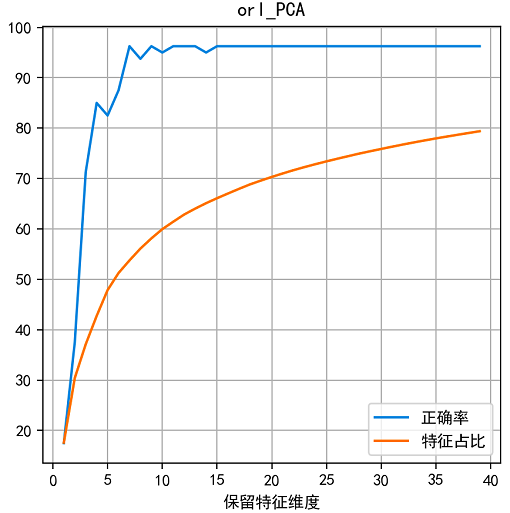
\includegraphics{Images/fig1.png}}
    \caption{ORL Set Using PCA+KNN Method}
    \label{fig1}
    \end{figure}

\begin{figure}[htb]
    \centerline{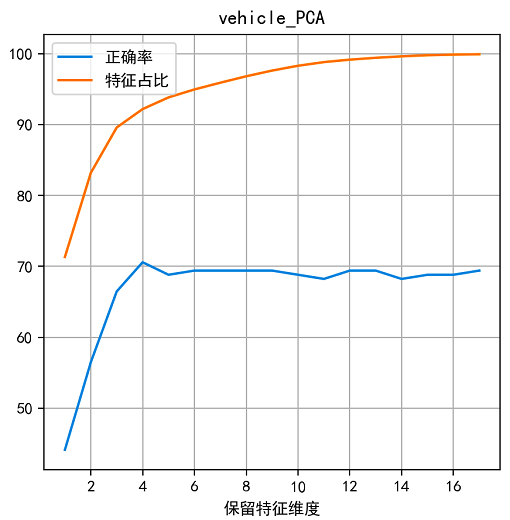
\includegraphics{Images/fig2.png}}
    \caption{Vehicle Set Using PCA+KNN Method}
    \label{fig2}
    \end{figure} \par
$\mathbf{LDA}$方法:
\begin{figure}[htb]
    \centerline{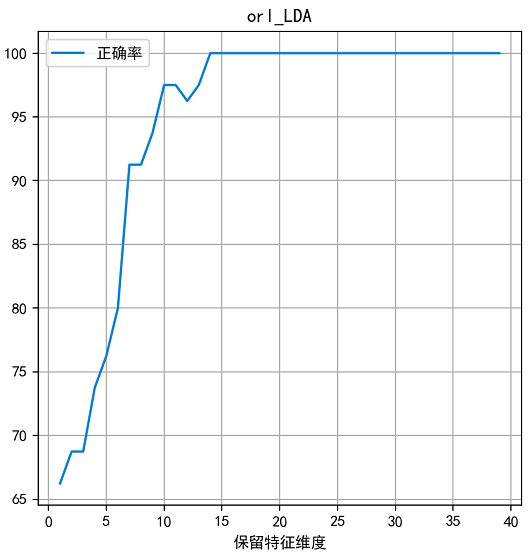
\includegraphics{Images/fig3.png}}
    \caption{ORL Set Using LDA+KNN Method}
    \label{fig3}
    \end{figure}

\begin{figure}[htb]
    \centerline{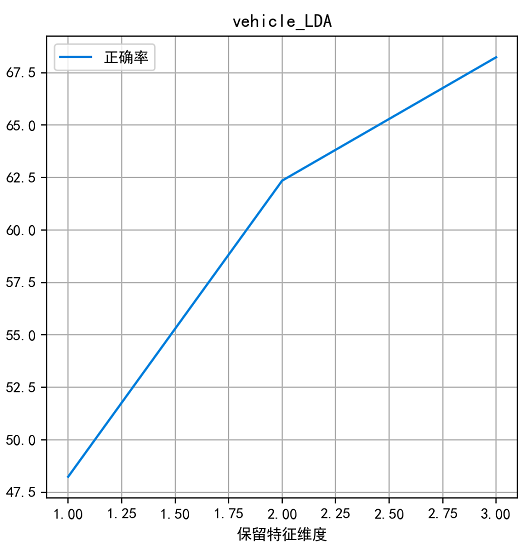
\includegraphics{Images/fig4.png}}
    \caption{Vehicle Set Using LDA+KNN Method}
    \label{fig4}
    \end{figure} \par

\end{CJK}

\clearpage

\section{Appendix}
\begin{CJK}{UTF8}{gkai}
    本次作业中,所采用的拟合计算代码均是基于Matlab和Python3.9,相关的源码已经被开源于Github上:
    \url{https://github.com/Alexiopro/First-year-of-UCAS/tree/main/UCAS/Source%20Code%20of%20Pattern%20Classification}
    供读者查用。 \par
\end{CJK}
\end{document}
